\documentclass{article}

\usepackage{graphicx}
\usepackage[utf8]{inputenc}
\usepackage[T1]{fontenc}
\usepackage[francais]{babel}
\usepackage{hyperref}
\usepackage{amsmath,amsfonts,amssymb}
\usepackage{Tkz-Tab}
\usepackage{wrapfig}
\usepackage{Verbatim}

\begin{document}

\title{Gestion de flux dans le réseau
	\smallbreak
	TD n\degre4
	\smallbreak
	Modélisation mathématique
	\smallbreak
	Q4}
\author{Sibylle Roux \and Juliette Arazo \and Nicolas Le Gallo \and Tanguy Thomas}


\maketitle

\newpage

\tableofcontents

\newpage

\part{Etude statistiques}

\section{Etude statistique des temps interarrivés pour tous les serveurs}

\subsection{Indicateurs de position et de dispersion}

\subsection{Fonction de répartition}

\subsection{Histogramme}


\section{Etude statistique des temps interarrivés pour le serveur 1}

\subsection{Indicateurs de position et de dispersion}

\subsection{Fonction de répartition}

\subsection{Histogramme}

\paragraph{Histogramme}
\begin{center}
%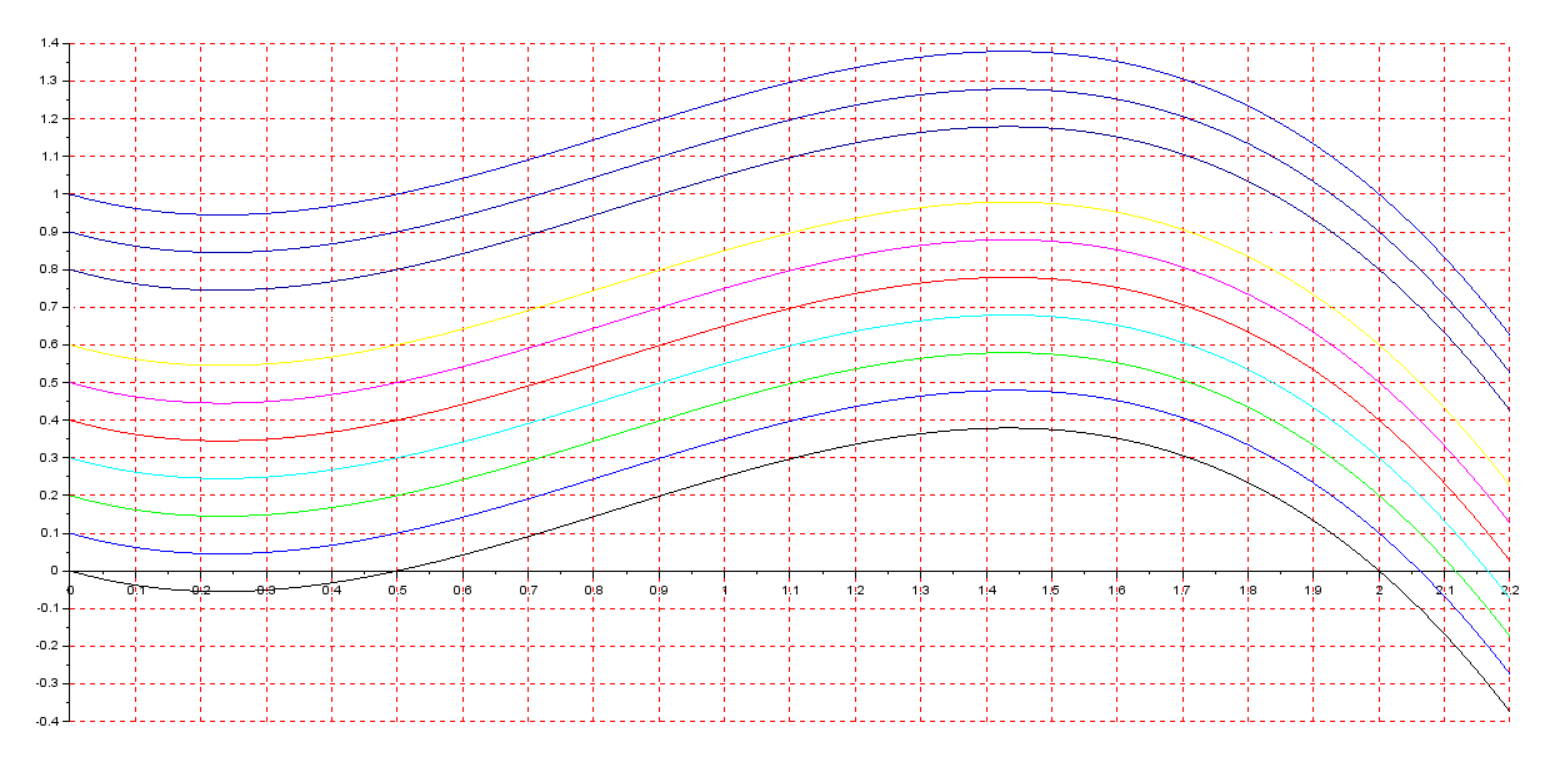
\includegraphics[width=300px]{img/part1/AlleeI.png}
\end{center}
\paragraph{}



\section{Etude statistique des temps interarrivés pour le serveur 2}

\subsection{Indicateurs de position et de dispersion}

\subsection{Fonction de répartition}

\subsection{Histogramme}


\section{Etude statistique des temps interarrivés pour le serveur 3}

\subsection{Indicateurs de position et de dispersion}

\subsection{Fonction de répartition}

\subsection{Histogramme}


\part{Ajustement graphique à des lois mathématique}

\section{Tous les serveurs}

\subsection{Ajustement à la loi uniforme}

\subsubsection{Estimation des paramètres}
\subsubsection{Superposition de la fonction de répartition}
\subsubsection{Superposition de la fonction de densité et de l'histogramme}

\subsection{Ajustement à la loi normale}

\subsubsection{Estimation des paramètres}
\subsubsection{Superposition de la fonction de répartition}
\subsubsection{Superposition de la fonction de densité et de l'histogramme}

\subsection {Ajustement à la loi exponentielle}

\subsubsection{Estimation des paramètres}
\subsubsection{Superposition de la fonction de répartition}
\subsubsection{Superposition de la fonction de densité et de l'histogramme}

\section{Serveur 1}

\subsection{Ajustement à la loi uniforme}

\subsubsection{Estimation des paramètres}
\subsubsection{Superposition de la fonction de répartition}
\subsubsection{Superposition de la fonction de densité et de l'histogramme}

\subsection{Ajustement à la loi normale}

\subsubsection{Estimation des paramètres}
\subsubsection{Superposition de la fonction de répartition}
\subsubsection{Superposition de la fonction de densité et de l'histogramme}

\subsection {Ajustement à la loi exponentielle}

\subsubsection{Estimation des paramètres}
\subsubsection{Superposition de la fonction de répartition}
\subsubsection{Superposition de la fonction de densité et de l'histogramme}

\section{Serveur 2}

\subsection{Ajustement à la loi uniforme}

\subsubsection{Estimation des paramètres}
\subsubsection{Superposition de la fonction de répartition}
\subsubsection{Superposition de la fonction de densité et de l'histogramme}

\subsection{Ajustement à la loi normale}

\subsubsection{Estimation des paramètres}
\subsubsection{Superposition de la fonction de répartition}
\subsubsection{Superposition de la fonction de densité et de l'histogramme}

\subsection {Ajustement à la loi exponentielle}

\subsubsection{Estimation des paramètres}
\subsubsection{Superposition de la fonction de répartition}
\subsubsection{Superposition de la fonction de densité et de l'histogramme}

\section{Serveur 3}

\subsection{Ajustement à la loi uniforme}

\subsubsection{Estimation des paramètres}
\subsubsection{Superposition de la fonction de répartition}
\subsubsection{Superposition de la fonction de densité et de l'histogramme}

\subsection{Ajustement à la loi normale}

\subsubsection{Estimation des paramètres}
\subsubsection{Superposition de la fonction de répartition}
\subsubsection{Superposition de la fonction de densité et de l'histogramme}

\subsection {Ajustement à la loi exponentielle}

\subsubsection{Estimation des paramètres}
\subsubsection{Superposition de la fonction de répartition}
\subsubsection{Superposition de la fonction de densité et de l'histogramme}

\newpage
\appendix

\section{}

\subsection{}

\subsubsection{}

\begin{verbatim}
\end{verbatim}

\end{document}